\documentclass[a4paper]{article}   	% use "amsart" instead of "article" for AMSLaTeX format

\usepackage{geometry}               	
\geometry{a4paper,margin=1.1in}           % ... or a4paper or a5paper or ... 

%\usepackage{graphicx}			

\usepackage{amsmath}
\usepackage{tikz}

\usepackage{hyperref}
\hypersetup{colorlinks=true,
    citecolor=blue,    filecolor=blue,
    linkcolor=blue,     urlcolor=blue
}
\usepackage{cite}

\newcommand{\ir}{\frac{1}{r}}
\newcommand{\Integ}[1]{\int_{-\infty}^{\infty} \!\!\!\!\!
  \mathrm{d}#1}
\newcommand{\RInteg}[1]{\int_{0}^{\infty} \!\!\!\!\! #1\mathrm{d}#1}
\newcommand{\rInteg}{\int_{0}^{r_{max}} \!\!\!\!\! r\mathrm{d}r}
\newcommand{\TInteg}[1]{\int_{0}^{2\pi} \!\!\!\!\! \mathrm{d}#1}

\newcommand{\tB}[2]{\tilde{B}_{#1,m}^{#2}}
\newcommand{\tE}[2]{\tilde{E}_{#1,m}^{#2}}
\newcommand{\tj}[2]{\tilde{j}_{#1,m}^{#2}}

\newcommand{\trho}[1]{\tilde{\rho}_{m}^{#1}}

% Reference automatique aux equations, sections, figures
\usepackage{cleveref}

\title{A pseudo-spectral, cylindrical and dispersion-free Particle-In-Cell algorithm}
%\pagestyle{empty}
\author{R\'emi \textsc{Lehe}}

\begin{document}

\maketitle


\section*{Introduction (rough ideas)}

\paragraph{Importance of PIC codes } Used in many fields : astro, laser-plasma interaction. However, 3D codes are expensive, and their limited resolution leads to many numerical effects (Cherenkov, dispersion).

\paragraph{Cylindrical PIC codes} A range of physical situations have close-to cylindrical symmetry (e.g. electron beam propagation, laser-wakefield acceleration), and they can be simulated with very significant speedup using a cylindrically symmetric algorithm \cite{Lifschitz, Davidson}. This typically reduces the cost of the simulation to a few times that of a 2D simulation, instead of that of a full 3D simulation.

\paragraph{Spectral PIC codes} In parallel, 3D spectral PIC codes have been developped, and can mitigate numerical instability (articles Warren and Brendan Godfrey). In spectral space, some algorithms have no numerical dispersion whatsoever \cite{Haber}. This is important in laser-wakefield acceleration since even a very small amount of numerical dispersion can introduce spurious injection. Dispersion is also important when simulating beam physics, where lower-than-c propagation leads to Cherenkov effect and faster-than-c leads to fields unphysically traveling ahead of the beam. Typically, this imposes to strongly overresolve the wavelength of the laser (thereby increasing computational requirements), and to use very asymetric cell aspect ratio. Although the spectral algorithms reduce the requirements on the longitudinal resolution, they still require a 3D grid, and therefore a large computational load.

\paragraph{Spectral, cylindrical PIC codes } In this document, we combine the two approaches. Advantages:
\begin{itemize}
\item Significant speedup due to the cylindrical geometry, and the
  lower number of particles.
\item Ideal dispersion relation in PSATD, independent on azimuthal mode (with a finite difference algorithm, the different modes go at different speeds)
\item Fields are colocated in space and time in PSATD and not
  staggered, which simplifies interpolation, and prevents
  time-interpolation errors in compensation of E and B (article plasma
  lens)
\item Time step can be bigger (but still need to resolve the
  oscillations of the particles in time).
\item Ability to apply filters in k space and thereby limit numerical instabilities
\item Prevent on-axis noise that appear in finite-difference cylindrical algorithms.
\end{itemize}


\section{Representation of the fields and continuous equations}

\subsection{Reminder on Cartesian spectral codes}

It is well-known that the Maxwell equations in Cartesian coordinates 
\begin{align}
\frac{1}{c^2}\partial_t E_x = \partial_y B_z - \partial_z B_y - \mu_0  j_x \qquad&   
\partial_t B_x = -\partial_y E_z + \partial_z E_y \label{eq:CartMaxwellx} \\
\frac{1}{c^2}\partial_t E_y = \partial_z B_x - \partial_x B_z - \mu_0  j_y \qquad &   
\partial_t B_y = -\partial_z E_x + \partial_x E_z \label{eq:CartMaxwelly}  \\
\frac{1}{c^2}\partial_t E_z = \partial_x B_y - \partial_y B_x - \mu_0  j_z \qquad &   
\partial_t B_z = -\partial_x E_y + \partial_y E_x \label{eq:CartMaxwellz} 
\end{align}
can be solved by representing the fields as a sum of Fourier modes.
\begin{equation}
\label{eq:CartBwTrans}
F_u(\vec{r}) = \frac{1}{(2\pi)^{3}}\Integ{k_x} \,\Integ{k_y}\, \Integ{k_z} \; \hat{F}_u(\vec{k}) e^{i(k_x x + k_y y + k_z z)} 
\end{equation}
with 
\begin{equation}
\label{eq:CartFwTrans}
\hat{F}_u(\vec{k})  = \Integ{x} \,\Integ{y}\, \Integ{z} \; F_u(\vec{r}) e^{-i(k_x x + k_y y + k_z z)} 
\end{equation}
where $F$ is any of the fields $E$, $B$ or $j$, and where $u$ is
either $x$, $y$ or $z$. In this case, the different Fourier modes decouple and the equations \cref{eq:CartMaxwellx,eq:CartMaxwelly,eq:CartMaxwellz} become 
\begin{align}
\frac{1}{c^2}\partial_t \hat{E}_x = ik_y \hat{B}_z - ik_z \hat{B}_y - \mu_0 \hat{j}_x \qquad &   
\partial_t \hat{B}_x = -ik_y \hat{E}_z + ik_z \hat{E}_y \\
\frac{1}{c^2}\partial_t \hat{E}_y = ik_z \hat{B}_x - ik_x \hat{B}_z - \mu_0  \hat{j}_y \qquad &   
\partial_t \hat{B}_y = -ik_z \hat{E}_x + ik_x \hat{E}_z \\
\frac{1}{c^2}\partial_t \hat{E}_z = ik_x \hat{B}_y - ik_y \hat{B}_x - \mu_0 \hat{j}_z  \qquad &   
\partial_t \hat{B}_z = -ik_x \hat{E}_y + ik_y \hat{E}_x 
\end{align}
The Fourier coefficients can then be integrated in time, and
transformed back into real space using \cref{eq:CartBwTrans}. This is
the core principle of Cartesian pseudo-spectral time-domain (PSTD)
codes and pseudo-spectral analytical time-domain (PSATD) codes.

\subsection{Cylindrical spectral decomposition}

The Fourier representation \cref{eq:CartBwTrans} is no longer the
appropriate representation when the Maxwell equations are written in cylindrical coordinates.
\begin{align}
\frac{1}{c^2}\partial_t E_r = \ir \partial_\theta B_z - \partial_z B_\theta - \mu_0  j_r \qquad&   
\partial_t B_r = -\ir \partial_\theta E_z + \partial_z E_\theta \label{eq:CircMaxwellr} \\
\frac{1}{c^2}\partial_t E_\theta = \partial_z B_r - \partial_r B_z - \mu_0  j_\theta \qquad &   
\partial_t B_\theta = -\partial_z E_r + \partial_r E_z \label{eq:CircMaxwellt}  \\
\frac{1}{c^2}\partial_t E_z = \ir\partial_r r B_\theta - \ir\partial_\theta B_r - \mu_0  j_z \qquad & 
\partial_t B_z = -\ir\partial_r r E_\theta + \ir\partial_\theta E_r \label{eq:CircMaxwellzz} 
\end{align}
When replacing
\cref{eq:CartBwTrans} into the \cref{eq:CircMaxwellr,eq:CircMaxwellt,eq:CircMaxwellzz}, the Fourier modes do not decouple. Instead one has to use the Fourier-Bessel representation.
\begin{align}
& F_z(\vec{r}) = \frac{1}{(2\pi)^2}\sum_{m=-\infty}^{\infty} \Integ{k_z}
\RInteg{k_\perp }\; \tilde{F}_{z,m}(k_z,k_\perp ) \; J_m(k_\perp r)\, e^{-im\theta + ik_z z} 
\label{eq:CircBwTransz} \\
& F_r(\vec{r}) = \frac{1}{(2\pi)^2}\sum_{m=-\infty}^{\infty} \Integ{k_z}\,\RInteg{k_\perp }\;
\left( \tilde{F}_{+,m}(k_z,k_\perp )\; J_{m+1}(k_\perp r) +\tilde{F}_{-,m}(k_z,k_\perp )\; J_{m-1}(k_\perp r)
\right)  e^{-im\theta +ik_z z}
\label{eq:CircBwTransr} \\
& F_\theta(\vec{r}) = \frac{1}{(2\pi)^2}\sum_{m=-\infty}^{\infty} \Integ{k_z}\,\RInteg{k_\perp }\;
i\left( \tilde{F}_{+,m}(k_z,k_\perp )\; J_{m+1}(k_\perp r) - \tilde{F}_{-,m}(k_z,k_\perp )\; J_{m-1}(k_\perp r)
\right)  e^{-im\theta +ik_z z} 
\label{eq:CircBwTranst}
\end{align}
where $F$ is either $E$, $B$ or $j$. Notice that the Cartesian
component $F_z$ and cylindrical components
$F_r$, $F_\theta$ do not transform in the same manner, which is due
to their different behavior close to the axis. (See
\cref{sec:CircTrans} for a derivation of this representation and for
its relation to the Fourier transform.) In addition, the coefficients $\tilde{F}_z$, $\tilde{F}_+$ and
 $\tilde{F}_{-}$ are given by:
\begin{align}
\tilde{F}_{z,m}(k_z,k_\perp ) &= \Integ{z} \RInteg{r}
\TInteg{\theta} \;F_z(\vec{r})\; J_m(k_\perp r) e^{im\theta
 - i k_z z} \label{eq:CircFwTransz} \\
\tilde{F}_{+,m}(k_z,k_\perp ) &= \Integ{z} \RInteg{r}
\TInteg{\theta} \;\frac{F_r (\vec{r})-iF_\theta (\vec{r})}{2}\; J_{m+1}(k_\perp r) e^{im\theta
 - i k_z z} \label{eq:CircFwTransp} \\
\tilde{F}_{-,m}(k_z,k_\perp ) &= \Integ{z} \RInteg{r}
\TInteg{\theta} \;\frac{F_r (\vec{r})+iF_\theta(\vec{r})}{2}\; J_{m-1}(k_\perp r) e^{im\theta
 - i k_z z} \label{eq:CircFwTransm} 
\end{align}
\noindent Note also that scalar fields (like $\rho$) transform in the same way as the Cartesian component $F_z$.

When replacing \cref{eq:CircBwTransr,eq:CircBwTranst,eq:CircBwTransz} into the Maxwell equations in cylindrical
coordinates \cref{eq:CircMaxwellr,eq:CircMaxwellt,eq:CircMaxwellzz},
the different modes decouple, and the equations for the spectral
coefficients become:
\begin{align}
\frac{1}{c^2}\partial_t \tilde{E}_{+,m} = - \frac{ik_\perp }{2}\tilde{B}_{z,m} + k_z\tilde{B}_{+,m} - \mu_0\tilde{j}_{+,m} \qquad &   
\partial_t \tilde{B}_{+,m} = \frac{ik_\perp }{2} \tilde{E}_{z,m} - k_z
\tilde{E}_{+,m} 
\label{eq:CircMaxwellp} \\
\frac{1}{c^2}\partial_t \tilde{E}_{-,m} = -\frac{ik_\perp }{2} \tilde{B}_{z,m} - k_z \tilde{B}_{-,m} - \mu_0  \tilde{j}_{-,m} \qquad &   
\partial_t \tilde{B}_{-,m} = \frac{ik_\perp }{2} \tilde{E}_{z,m} + k_z
\tilde{E}_{-,m} \label{eq:CircMaxwellm} \\
\frac{1}{c^2}\partial_t \tilde{E}_{z,m} = ik_\perp  \tilde{B}_{+,m} + ik_\perp \tilde{B}_{-,m}  - \mu_0 \tilde{j}_{z,m}  \qquad & 
\partial_t \tilde{B}_{z,m} = -ik_\perp  \tilde{E}_{+,m} - ik_\perp \tilde{E}_{-,m}  \label{eq:CircMaxwellz} 
\end{align}
(See \cref{sec:SpectMaxwell} for a derivation of these equations.) In
addition, the conservation equations
$\vec{\nabla}\cdot\vec{E}=\rho/\epsilon_0$ and
$\vec{\nabla}\cdot\vec{B} = 0$
become
\begin{equation}
\label{eq:SpectCons}
k_\perp (\tilde{E}_{+,m} -\tilde{E}_{-,m}) + ik_z \tilde{E}_{z,m} =
\frac{\tilde{\rho}_m}{\epsilon_0} \qquad
 k_\perp (\tilde{B}_{+,m} -\tilde{B}_{-,m}) + ik_z \tilde{B}_{z,m} =
0 \end{equation}
As expected, the above conservation equations are
preserved by the Maxwell equations
\cref{eq:CircMaxwellp,eq:CircMaxwellm,eq:CircMaxwellz}, provided
that the current satisfies $\partial_t
\rho + \vec{\nabla} \cdot \vec{j} = 0$, i.e. in spectral space:
\begin{equation}
\label{eq:SpectCharge}
\partial_t \tilde{\rho}_m + k_\perp (\tilde{j}_{+,m} -\tilde{j}_{-,m}) + ik_z
\tilde{j}_{z,m} = 0
\end{equation}  

Again, the equations \cref{eq:CircMaxwellp,eq:CircMaxwellm,eq:CircMaxwellz}  can be
integrated in time, and the fields can then be transformed back into
real space, using \cref{eq:CircBwTransz,eq:CircBwTransr,eq:CircBwTranst}. Notice that
the structure of \cref{eq:CircMaxwellp,eq:CircMaxwellm,eq:CircMaxwellz} is similar to
the structure of the corresponding equations in a Cartesian PIC code. Therefore,
the methods used to integrate the fields in time in a Cartesian
spectral code (e.g. PSATD) should be transposable to the cylindrical case.

Typically one needs only a few modes in $m$, therefore the fields are
reduced to a few 2D tables $\tilde{F}_m(k_z,k_\perp )$ instead of the
3D tables $\hat{F}(k_x,k_y,k_z)$. (For instance, in a purely symmetric
case, there is only one mode: $m=0$.) In addition, since the fields
$F_z, F_r, F_\theta$ are real, and since $J_m(x) =(-1)^mJ_{-m}(x)$ \cite{Abramowitz},
one has
\[ \tilde{F}_{z,-m}(k_z, k_\perp) = (-1)^m\tilde{F}_{z,m}^{*} (-k_z,
k_\perp) \qquad \tilde{F}_{+,-m}(k_z, k_\perp) =
(-1)^{m+1} \tilde{F}_{-,m}^{*} (-k_z, k_\perp) \]
This means that one only needs to study the evolution of the modes having $m\geq 0$, as the modes with $m<0$ can
be directly deduced from these fields.

\section{Numerical implementation}

\subsection{Overview of the algorithm}

The algorithm presented here uses the above-mentioned representation
of the fields. Although the fields are represented by a few
2D arrays, the particles are still distributed in 3D and their motion
is integrated in 3D. However, due to the
lower number of cells in a 2D array, one can drastically reduce the
total number of particles and still have significative statistics.

Similarly to a Cartesian pseudo-spectral code, we do not perform the
current deposition and field gathering directly from the
macroparticles to the spectral space. (This is inefficient since the
deposition and gathering are local operations in real space -- i.e. affect
only the few cells next to the macroparticle -- but global operations
in spectral space -- i.e. they affect all the spectral modes
simultaneously.) Instead we use an intermediate grid where these
operations can be performed locally, and where the fields $\mathcal{F}_{u,m}$
are defined by
\begin{equation} 
\label{eq:IntermBwTrans}
F_u(\vec{r}) = \sum_{m=-\infty}^{\infty} \mathcal{F}_{u,m}(r,z)
e^{-im\theta} 
\end{equation}
\begin{equation}
\label{eq:IntermFwTrans}
\mathcal{F}_{u,m}(r,z) = \frac{1}{2\pi} \TInteg{\theta} \;
F_u(\vec{r})e^{im\theta}
\end{equation}
where ${F}$ is either ${E}$, ${B}$ or
${j}$ and $u$ is either $z$, $r$ or $\theta$. Notice that this representation is the
same as that of \cite{Lifschitz, Davidson}. Notice also that, in this
representation, we kept the spectral decomposition in the azimuthal
direction, since the factors $e^{im\theta}$ can be efficiently computed from the
particle positions by using the relation $e^{im\theta} = (x+iy)^m/r^m$
\cite{Lifschitz}.

After the particles deposit their charge and current onto this grid,
the fields of the intermediate grid are transformed into spectral
space where the Maxwell equations can be easily integrated. From
\cref{eq:IntermFwTrans,eq:IntermBwTrans} and
\cref{eq:CircFwTransz,eq:CircFwTransp,eq:CircFwTransm,eq:CircBwTransz,eq:CircBwTransr,eq:CircBwTranst}, the transformation between these
representations is:
\begin{align*}
\tilde{F}_{z,m}(k_z,k_\perp) & = \mathrm{FT} [ \; \mathrm{HT}_{m}
                               [ \; \mathcal{F}_{z,m}(r,z) \; ] \;]\\
\tilde{F}_{+,m}(k_z,k_\perp) &= \mathrm{FT} \left[ \; \mathrm{HT}_{m+1} \left[ \frac{
  \mathcal{F}_{r,m} -i  \mathcal{F}_{\theta,m} }{2}  \right] \;\right] \\
\tilde{F}_{-,m}(k_z,k_\perp) &= \mathrm{FT} \left[ \; \mathrm{HT}_{m-1} \left[ \frac{
  \mathcal{F}_{r,m} +i  \mathcal{F}_{\theta,m} }{2}  \right] \;\right] 
\end{align*}
and
\begin{align*}
\mathcal{F}_{z,m}(r,z) &= \mathrm{IFT} [\; \mathrm{IHT}_{m} [
                         \tilde{F}_{z,m}(k_z,k_\perp) ] \; ] \\
\mathcal{F}_{r,m}(r,z) & = \mathrm{IFT} \left[ \; \mathrm{IHT}_{m+1}
                         [ \tilde{F}_{+,m}(k_z,k_\perp) ] + \mathrm{IHT}_{m-1} [
                         \tilde{F}_{-,m}(k_z,k_\perp) ] \; \right] \\
\mathcal{F}_{\theta,m}(r,z) & = i\;\mathrm{IFT} \left[ \; \mathrm{IHT}_{m+1}
                         [ \tilde{F}_{+,m}(k_z,k_\perp) ] - \mathrm{IHT}_{m-1} [ \tilde{F}_{-,m}(k_z,k_\perp) ] \; \right]
\end{align*}
where $\mathrm{FT}$ represents a Fourier Transform along the $z$
axis and $\mathrm{HT}_{n}$ represents a Hankel Transform of order
$n$ along the $r$ axis, and where $\mathrm{IFT}$ and
$\mathrm{IHT}_{n}$ represent the corresponding inverse
transformations:
\[ \mathrm{FT} [f]\, (k_z) \equiv \Integ{z} \, e^{-ik_zz} \; f(z) \qquad 
\mathrm{IFT} [g] \,(z)\equiv \frac{1}{2\pi}\Integ{k_z} \, e^{ik_zz} \;  g(k_z)\]
\[ \mathrm{HT}_{n} [f]\,(k_\perp) \equiv 2\pi \RInteg{r} \,
J_{n}(k_\perp r) \; f(r) \qquad 
\mathrm{IHT}_{n} [g]\,(r) \equiv \frac{1}{2\pi}\RInteg{k_\perp} \,  J_{n}(k_\perp r)  \;  g(k_\perp) \]

The above equations show that the transformation from the intermediate
grid ($\mathcal{F}_{u,m}$) to the spectral grid ($\tilde{F}_{u,m}$) is
the combination of a Fourier transform (in $z$) and a Hankel transform
(in $r$). The Fourier transform in $z$ can be implemented through a Fast Fourier
Transform (FFT) algorithm, which requires the intermediate and spectral grid to
have regular spacing in $z$ and $k_z$ respectively. On the other hand,
there are a variety of existing algorithms (that are not mathematically
equivalent) to discretize the Hankel
transform (e.g. \cite{Cree,Yu,Siegman,Guizar,KaiMing}), and the use of one or the other
is very dependent of the particular application pursued. Broadly
speaking, most Discrete Hankel Transform (DHT) algorithms consists in 
\begin{enumerate}
\item Choosing a discrete grid in $r$ and $k_\perp$ space, on which to
  sample the functions to be transformed. In some algorithms, these
  grids may not be regularly spaced, and can be for instance
  logarithmically spaced \cite{Siegman} or correspond to the zeros of
  Bessel functions \cite{Yu,Guizar,KaiMing}.
\item Once a grid is chosen, the DHT amouts to a linear operation on a
  finite set of points (the points of the grid) and can thus be
  represented by a matrix. Thus the second choice is that of a matrix
  that represents (as closely as possible), the exact Hankel Transform.
\end{enumerate}
Here, we choose to discretize the algorithm on a regular grid in
space
\[ r_j = \Delta r \left( j+\frac{1}{2} \right) \qquad  j \in \{0, ...,
N_r-1 \} \qquad \mathrm{where} \quad \Delta r = \frac{r_{max}}{N_r} \]
(Notice that neither $r=0$, nor $r=r_{max}$ are part of the grid.)
but on a non-regular grid in $k$ space. This is because the authorized
$k$ are determined by the boundary conditions, in the same way that
the periodic boundaries in a Cartesian code impose the use of
regularly-space $k$. Here, for simplicity, we impose that the
longitudinal fields be $0$ at $r_{max}$ (i.e. $E_z(r_{max}, z) = 0$,
$B_z(r_{max}, z) = 0$). In this case, it turns out that the set of authorized
$k_\perp$ depend on the mode $m$ and reads
\[  k^m_{\perp,j} = \frac{\alpha_j^m}{r_{max}} \qquad j \in \{0, ..., N_r-1 \}\]
where $\alpha^m_j$ is the $j$th positive zero of the Bessel function of order
$m$ $J_m$ (including the trivial value $\alpha_0^m=0$ for
$m>0$). These values are represented in figure \ref{fig:Kgrid}. Notice
that the fact that the $k$s depend on the mode number $m$ is not a
problem since each mode evolves separately in
\cref{eq:CircMaxwellp,eq:CircMaxwellm,eq:CircMaxwellz}.

\begin{figure}[!h]
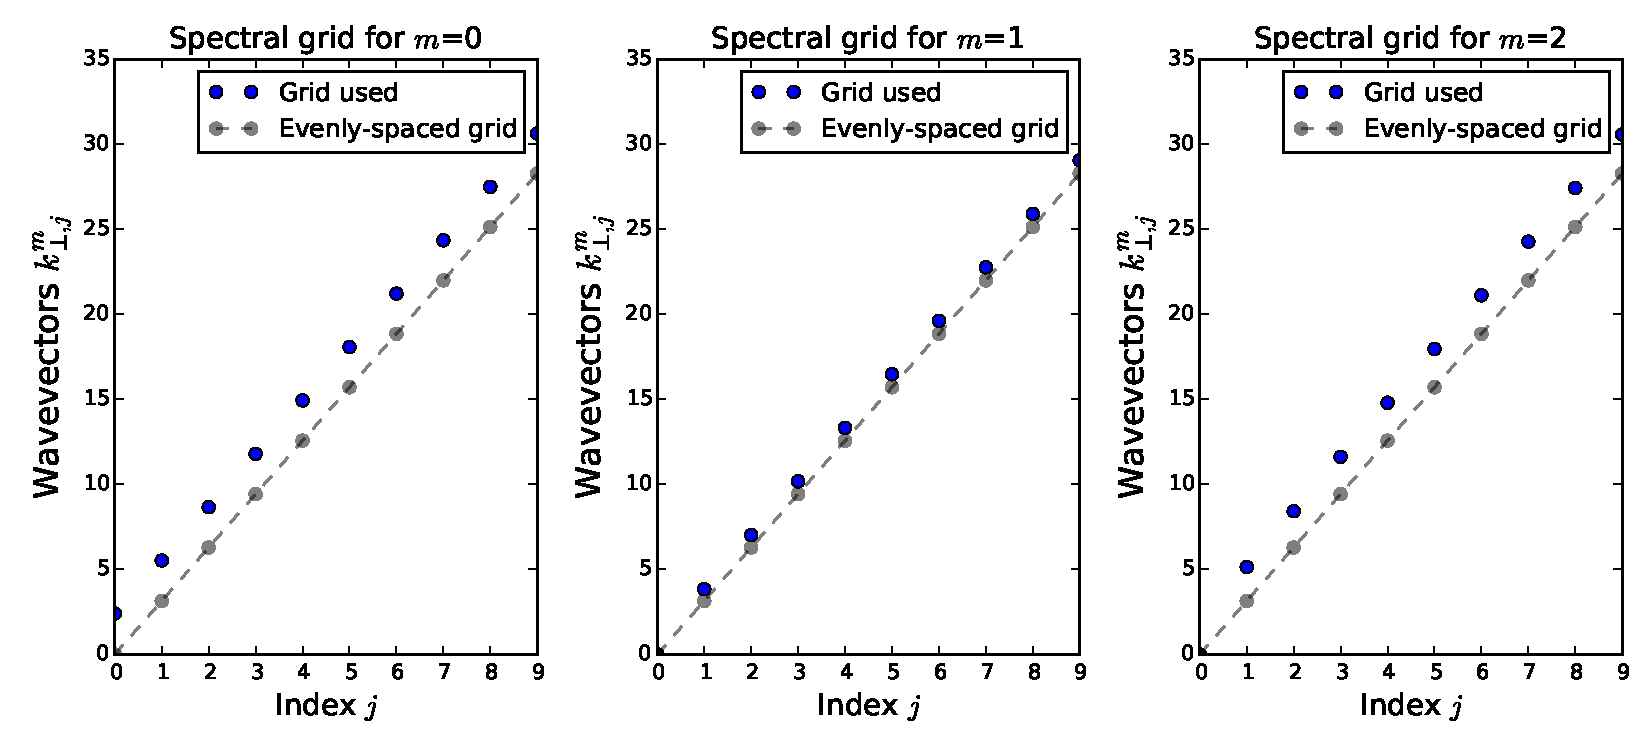
\includegraphics[width=\textwidth]{KGrid.pdf}
\caption{\label{fig:Kgrid}Position of the grid points in $k$ space
  (blue dots) for the azimuthal modes $m=0$, $m=1$ and $m=2$ for $N_r
  = 10$ and $r_{max}=1$. These values are compared with those of a
  regularly-spaced grid used in Cartesian spectral codes (grey dots, $k_j = j\pi/r_{max}$)}
\end{figure}

Once this grid is set up, the discrete hankel transform is simply a
linear operation on a finite set of points, and can thus be
represented by a matrix operation
\[ \mathrm{DHT^m_n}[f] \,(k^m_j) = \sum_{p=0}^{N_r-1} (M_{n,m})_{j,p}
\,f(r_p) \qquad \mathrm{IDHT^m_n}[g] \, (r_j) = \sum_{p=0}^{N_r-1}
(M^{-1}_{n,m})_{j,p} \,g(k^m_p) \]

Notice that the $N_r\times N_r$ transformation matrices $M_{n,m}$ and
$M_{n,m}^{-1}$ depend on $n$ (order of the Hankel transform) and $m$
(index of the spectral grid $k^m_j$ on which the Hankel transform is calculated). The expression of these matrices,
for the DHT algorithm that we chose, is given in
\cref{sec:HTMatrix}. %This particular choice is very specific and
%dependent on the imposed boundary conditions at $r_{max}$ ; in future
%work, different implementations of the DHT could be used depending on
%the boundary conditions. 
In practice, $M_{n,m}$ and $M^{-1}_{n,m}$ need to be
computed only once (at initialization), and can then be used at each
iteration. Notice also that the computational time for this
matrix multiplication is proportional to $N_r^2$, which is slow
compared to an FFT ($\propto N_r \log(N_r)$), but
still faster than the 2D FFT ($\propto N_x N_y \log(N_x) + N_x N_y \log(N_y) $)
which is used in a Cartesian spectral code. In practice, for $N_x = N_y =
N_r = 1000$ for instance, the DHT can be 50 times faster than a 2D FFT \cite{Norfolk}.

\Cref{fig:GlobalScheme} sums up the steps of the PIC cycle, including the
respective role of the intermediate and spectral grid. Note that, in the PSATD
scheme that we chose (and which is described in more details in
\cref{sec:FieldIntegration}), all the fields are defined at integer
timesteps, except for the currents, which are defined at half
timesteps. The following section describe the successive steps of the cycle in more details.

\begin{figure}

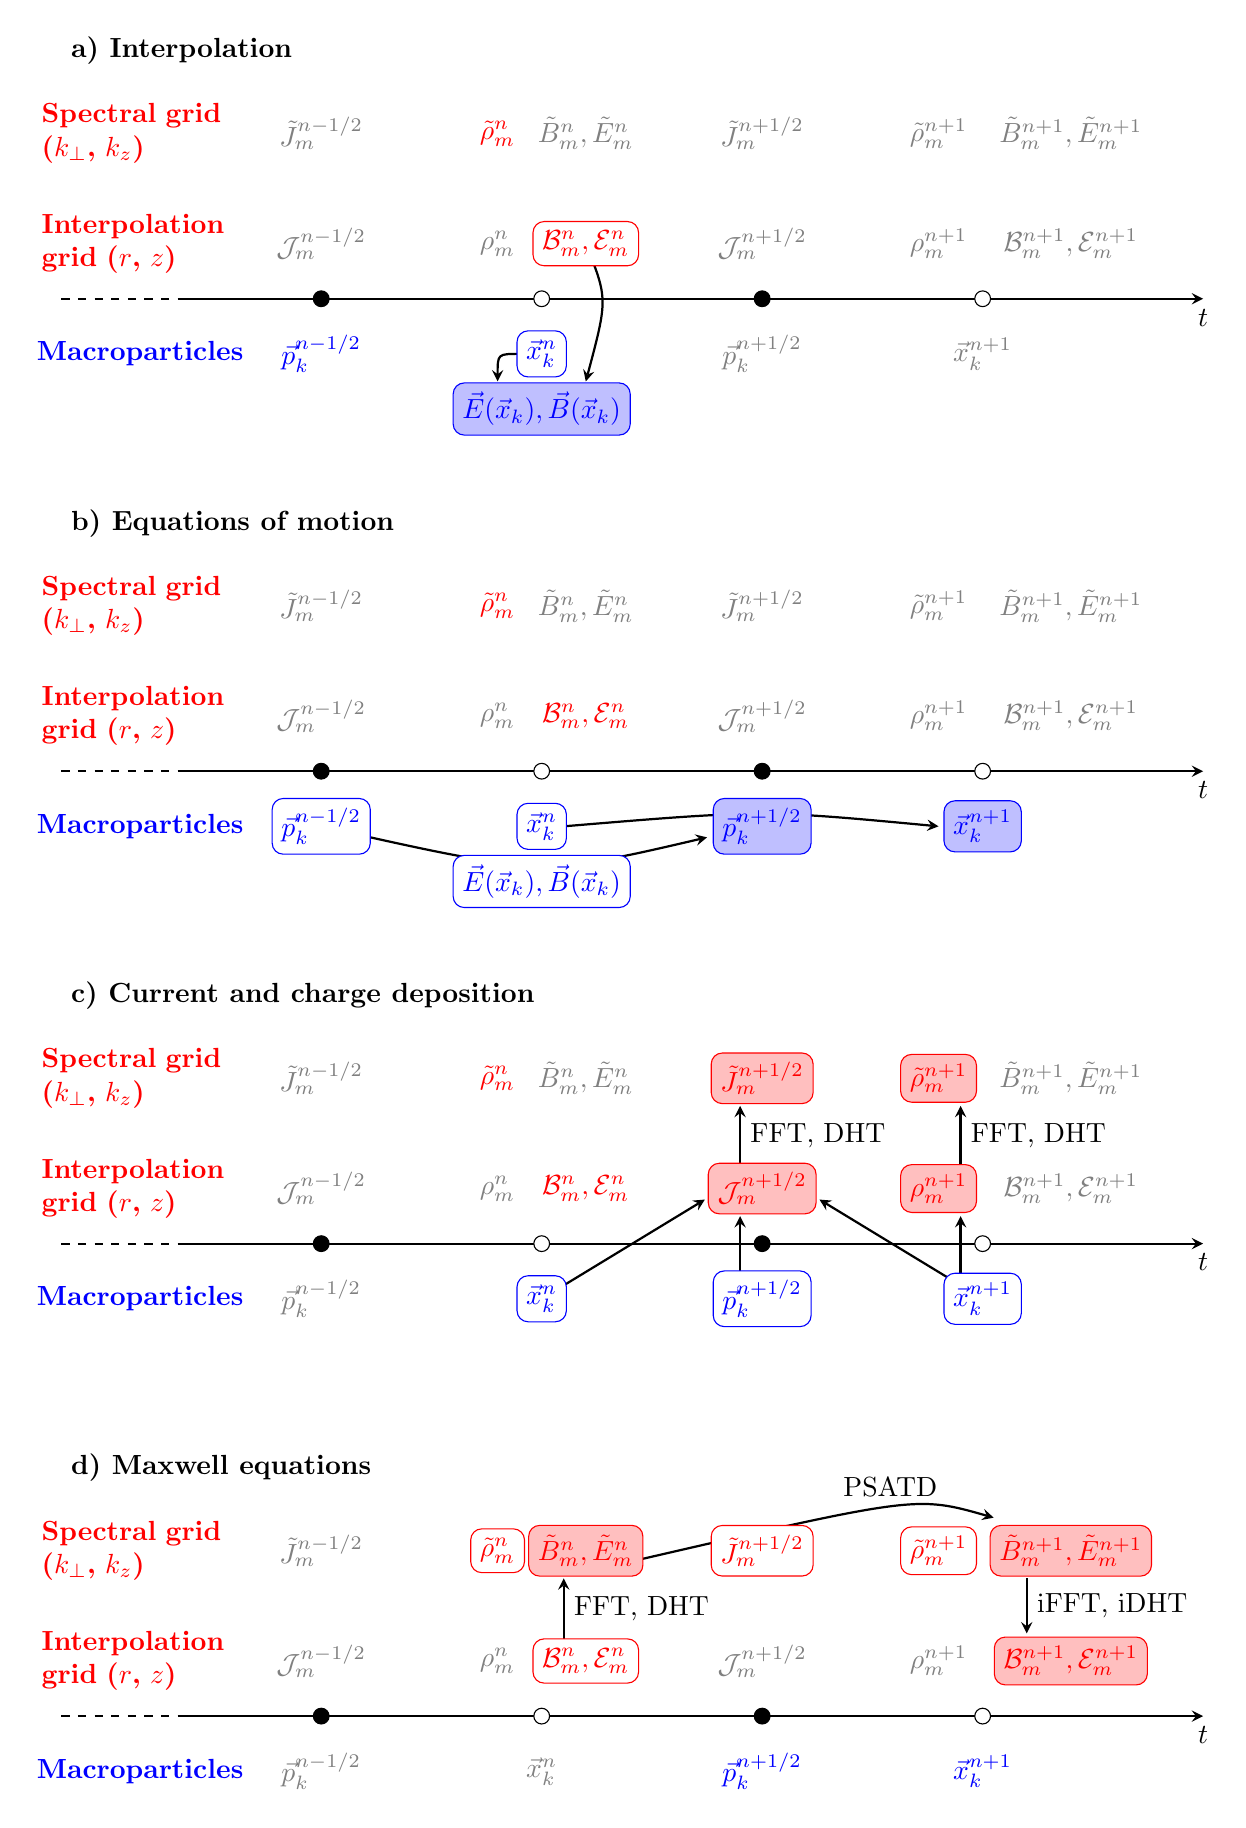
\begin{tikzpicture}
\def \Dt{2.8}
\def \yspac{0.7}

\begin{scope}[yshift=0cm]

\draw (-0.5,4.5*\yspac) node[anchor=west]{\textbf{a) Interpolation}};

% Axes
\draw[thick,->,>=stealth] (1,0) -- (5*\Dt,0) node[below]{$t$};
\draw[thick,dashed] (-0.5,0) -- (1,0);
% Labels
\draw (0.5,3*\yspac) node[red,text width=2.5cm]{\textbf{Spectral grid ($k_\perp$, $k_z$)}};
\draw (0.5,\yspac) node[red,text width=2.5cm]{\textbf{Interpolation grid ($r$, $z$)}};
\draw (0.5,-\yspac) node[blue]{\textbf{Macroparticles}};
% Timesteps
\foreach \n in {1,3} 
\draw[fill=black] (\n*\Dt,0) circle(0.1);
\foreach \n in {2,4} 
\draw[fill=white] (\n*\Dt,0) circle(0.1);
% Arrows
%\draw[->,>=stealth,thick] (3*\Dt,\yspac) -- (2.5*\Dt,-0.25);
%\draw[->,>=stealth,thick] (1.85*\Dt,\yspac) -- (1.85*\Dt,-0.25);
\draw[->,>=stealth,thick] (2.2*\Dt,\yspac) .. controls (2.3*\Dt,0) .. (2.2*\Dt,-1.5*\yspac);
\draw[->,>=stealth,thick] (1.9*\Dt,-1*\yspac) .. controls (1.8*\Dt,-1*\yspac) .. (1.8*\Dt,-1.5*\yspac);
% Fields
% -- n-1/2
\draw (\Dt,3*\yspac) node[gray,fill=white,draw=white,rounded corners]{$ \tilde{J}^{n-1/2}_m$};
\draw (\Dt,1*\yspac) node[gray,fill=white,draw=white,rounded corners]{$ \mathcal{J}^{n-1/2}_m$};
\draw (\Dt,-\yspac) node[blue]{$\vec{p}_k^{n-1/2}$};
% -- n
\draw (1.8*\Dt,3*\yspac) node[red,fill=white,draw=white,rounded corners]{$\tilde{\rho}^n_m$};
\draw (2.2*\Dt,3*\yspac) node[gray,fill=white,draw=white,rounded corners]{$  \tilde{B}^{n}_m, \tilde{E}^{n}_m$};
\draw (1.8*\Dt,\yspac) node[gray,fill=white,draw=white,rounded corners]{$\mathcal{\rho}^n_m$};
\draw (2.2*\Dt,\yspac) node[red,fill=white,draw=red,rounded corners]{$\mathcal{B}^{n}_m, \mathcal{E}^{n}_m$};
\draw (2*\Dt,-\yspac) node[blue,fill=white,draw=blue,rounded corners]{$\vec{x}_k^{n}$};
\draw (2*\Dt,-2*\yspac) node[blue,fill=white!75!blue,draw=blue,rounded corners]{$\vec{E}(\vec{x}_k), \vec{B}(\vec{x}_k)$};
% -- n+1/2
\draw (3*\Dt,3*\yspac) node[gray,fill=white,draw=white,rounded corners]{$ \tilde{J}^{n+1/2}_m$};
\draw (3*\Dt,1*\yspac) node[gray,fill=white,draw=white,rounded corners]{$ \mathcal{J}^{n+1/2}_m$};
\draw (3*\Dt,-\yspac) node[gray]{$\vec{p}_k^{n+1/2}$};
% -- n+1
\draw (3.8*\Dt,3*\yspac) node[gray,fill=white,draw=white,rounded corners]{$\tilde{\rho}^{n+1}_m$};
\draw (4.4*\Dt,3*\yspac) node[gray,fill=white,draw=white,rounded corners]{$  \tilde{B}^{n+1}_m, \tilde{E}^{n+1}_m$};
\draw (3.8*\Dt,\yspac) node[gray,fill=white,draw=white,rounded corners]{$\mathcal{\rho}^{n+1}_m$};
\draw (4.4*\Dt,\yspac) node[gray,fill=white,draw=white,rounded corners]{$\mathcal{B}^{n+1}_m, \mathcal{E}^{n+1}_m$};
\draw (4*\Dt,-\yspac) node[gray]{$\vec{x}_k^{n+1}$};

\end{scope}

\begin{scope}[yshift=-6cm]

\draw (-0.5, 4.5*\yspac) node[anchor=west]{\textbf{b) Equations of motion}};
% Axes
\draw[thick,->,>=stealth] (1,0) -- (5*\Dt,0) node[below]{$t$};
\draw[thick,dashed] (-0.5,0) -- (1,0);
% Labels
\draw (0.5,3*\yspac) node[red,text width=2.5cm]{\textbf{Spectral grid ($k_\perp$, $k_z$)}};
\draw (0.5,\yspac) node[red,text width=2.5cm]{\textbf{Interpolation grid ($r$, $z$)}};
\draw (0.5,-\yspac) node[blue]{\textbf{Macroparticles}};
% Timesteps
\foreach \n in {1,3} 
\draw[fill=black] (\n*\Dt,0) circle(0.1);
\foreach \n in {2,4} 
\draw[fill=white] (\n*\Dt,0) circle(0.1);
% Arrows
%\draw[->,>=stealth,thick] (\Dt,\yspac) -- (1.5*\Dt,-0.25);
%\draw[->,>=stealth,thick] (3*\Dt,\yspac) -- (2.5*\Dt,-0.25);
%\draw[->,>=stealth,thick] (1.85*\Dt,\yspac) -- (1.85*\Dt,-0.25);
\draw[->,>=stealth,thick] (1*\Dt,-\yspac) .. controls (2*\Dt,-1.9*\yspac) .. (2.75*\Dt,-1.2*\yspac);
\draw[->,>=stealth,thick] (2.1*\Dt,-1*\yspac) .. controls (3*\Dt,-0.7*\yspac) .. (3.8*\Dt,-1.*\yspac);
% Fields
% -- n-1/2
\draw (\Dt,3*\yspac) node[gray,fill=white,draw=white,rounded corners]{$ \tilde{J}^{n-1/2}_m$};
\draw (\Dt,1*\yspac) node[gray,fill=white,draw=white,rounded corners]{$ \mathcal{J}^{n-1/2}_m$};
\draw (\Dt,-\yspac) node[blue,fill=white,draw=blue,rounded corners]{$\vec{p}_k^{n-1/2}$};
% -- n
\draw (1.8*\Dt,3*\yspac) node[red,fill=white,draw=white,rounded corners]{$\tilde{\rho}^n_m$};
\draw (2.2*\Dt,3*\yspac) node[gray,fill=white,draw=white,rounded corners]{$  \tilde{B}^{n}_m, \tilde{E}^{n}_m$};
\draw (1.8*\Dt,\yspac) node[gray,fill=white,draw=white,rounded corners]{$\mathcal{\rho}^n_m$};
\draw (2.2*\Dt,\yspac) node[red,fill=white,draw=white,rounded corners]{$\mathcal{B}^n_m, \mathcal{E}^{n}_m$};
\draw (2*\Dt,-\yspac) node[blue,fill=white,draw=blue,rounded corners]{$\vec{x}_k^{n}$};
\draw (2*\Dt,-2*\yspac) node[blue,fill=white,draw=blue,rounded corners]{$\vec{E}(\vec{x}_k), \vec{B}(\vec{x}_k)$};
% -- n+1/2
\draw (3*\Dt,3*\yspac) node[gray,fill=white,draw=white,rounded corners]{$ \tilde{J}^{n+1/2}_m$};
\draw (3*\Dt,1*\yspac) node[gray,fill=white,draw=white,rounded corners]{$ \mathcal{J}^{n+1/2}_m$};
\draw (3*\Dt,-\yspac) node[blue,fill=white!75!blue,draw=blue,rounded corners]{$\vec{p}_k^{n+1/2}$};
% -- n+1
\draw (3.8*\Dt,3*\yspac) node[gray,fill=white,draw=white,rounded corners]{$\tilde{\rho}^{n+1}_m$};
\draw (4.4*\Dt,3*\yspac) node[gray,fill=white,draw=white,rounded corners]{$  \tilde{B}^{n+1}_m, \tilde{E}^{n+1}_m$};
\draw (3.8*\Dt,\yspac) node[gray,fill=white,draw=white,rounded corners]{$\mathcal{\rho}^{n+1}_m$};
\draw (4.4*\Dt,\yspac) node[gray,fill=white,draw=white,rounded corners]{$\mathcal{B}^{n+1}_m, \mathcal{E}^{n+1}_m$};
\draw (4*\Dt,-\yspac) node[blue,fill=white!75!blue,draw=blue,rounded corners]{$\vec{x}_k^{n+1}$};

\end{scope}

\begin{scope}[yshift=-12cm]

\draw (-0.5,4.5*\yspac) node[anchor=west]{\textbf{c) Current and charge deposition}};

% Axes
\draw[thick,->,>=stealth] (1,0) -- (5*\Dt,0) node[below]{$t$};
\draw[thick,dashed] (-0.5,0) -- (1,0);
% Labels
\draw (0.5,3*\yspac) node[red,text width=2.5cm]{\textbf{Spectral grid ($k_\perp$, $k_z$)}};
\draw (0.5,\yspac) node[red,text width=2.5cm]{\textbf{Interpolation grid ($r$, $z$)}};
\draw (0.5,-\yspac) node[blue]{\textbf{Macroparticles}};
% Timesteps
\foreach \n in {1,3} 
\draw[fill=black] (\n*\Dt,0) circle(0.1);
\foreach \n in {2,4} 
\draw[fill=white] (\n*\Dt,0) circle(0.1);
% Arrows
\draw[->,>=stealth,thick] (2*\Dt,-\yspac) -- (2.74*\Dt,0.8*\yspac);
\draw[->,>=stealth,thick] (2.9*\Dt,-\yspac) -- (2.9*\Dt,0.5*\yspac);
\draw[->,>=stealth,thick] (2.9*\Dt,1.4*\yspac) -- node[anchor=west]{FFT, DHT}(2.9*\Dt,2.5*\yspac);
\draw[->,>=stealth,thick] (4*\Dt,-\yspac) -- (3.26*\Dt,0.8*\yspac);
\draw[->,>=stealth,thick] (3.9*\Dt,-\yspac) -- (3.9*\Dt,0.5*\yspac);
\draw[->,>=stealth,thick] (3.9*\Dt,1.4*\yspac) -- node[anchor=west]{FFT, DHT}(3.9*\Dt,2.5*\yspac);
%\draw[->,>=stealth,thick] (3*\Dt,\yspac) -- (2.5*\Dt,-0.25);
%\draw[->,>=stealth,thick] (1.85*\Dt,\yspac) -- (1.85*\Dt,-0.25);
%\draw[->,>=stealth,thick] (1*\Dt,-\yspac) .. controls (2*\Dt,-1.9*\yspac) .. (2.75*\Dt,-1.2*\yspac);
%\draw[->,>=stealth,thick] (2.1*\Dt,-1*\yspac) .. controls (3*\Dt,-0.7*\yspac) .. (3.8*\Dt,-1.*\yspac);
% Fields
% -- n-1/2
\draw (\Dt,3*\yspac) node[gray,fill=white,draw=white,rounded corners]{$ \tilde{J}^{n-1/2}_m$};
\draw (\Dt,1*\yspac) node[gray,fill=white,draw=white,rounded corners]{$ \mathcal{J}^{n-1/2}_m$};
\draw (\Dt,-\yspac) node[gray,fill=white,draw=white,rounded corners]{$\vec{p}_k^{n-1/2}$};
% -- n
\draw (1.8*\Dt,3*\yspac) node[red,fill=white,draw=white,rounded corners]{$\tilde{\rho}^n_m$};
\draw (2.2*\Dt,3*\yspac) node[gray,fill=white,draw=white,rounded corners]{$  \tilde{B}^{n}_m, \tilde{E}^{n}_m$};
\draw (1.8*\Dt,\yspac) node[gray,fill=white,draw=white,rounded corners]{$\mathcal{\rho}^n_m$};
\draw (2.2*\Dt,\yspac) node[red,fill=white,draw=white,rounded corners]{$\mathcal{B}^n_m, \mathcal{E}^{n}_m$};
\draw (2*\Dt,-\yspac) node[blue,fill=white,draw=blue,rounded corners]{$\vec{x}_k^{n}$};
% -- n+1/2
\draw (3*\Dt,3*\yspac) node[red,fill=white!75!red,draw=red,rounded corners]{$ \tilde{J}^{n+1/2}_m$};
\draw (3*\Dt,1*\yspac) node[red,fill=white!75!red,draw=red,rounded corners]{$ \mathcal{J}^{n+1/2}_m$};
\draw (3*\Dt,-\yspac) node[blue,fill=white,draw=blue,rounded corners]{$\vec{p}_k^{n+1/2}$};
% -- n+1
\draw (3.8*\Dt,3*\yspac) node[red,fill=white!75!red,draw=red,rounded corners]{$\tilde{\rho}^{n+1}_m$};
\draw (4.4*\Dt,3*\yspac) node[gray,fill=white,draw=white,rounded corners]{$  \tilde{B}^{n+1}_m, \tilde{E}^{n+1}_m$};
\draw (3.8*\Dt,\yspac) node[red,fill=white!75!red,draw=red,rounded corners]{$\mathcal{\rho}^{n+1}_m$};
\draw (4.4*\Dt,\yspac) node[gray,fill=white,draw=white,rounded corners]{$\mathcal{B}^{n+1}_m, \mathcal{E}^{n+1}_m$};
\draw (4*\Dt,-\yspac) node[blue,fill=white,draw=blue,rounded corners]{$\vec{x}_k^{n+1}$};

\end{scope}

\begin{scope}[yshift=-18cm]

\draw (-0.5,4.5*\yspac) node[anchor=west]{\textbf{d) Maxwell equations}};

% Axes
\draw[thick,->,>=stealth] (1,0) -- (5*\Dt,0) node[below]{$t$};
\draw[thick,dashed] (-0.5,0) -- (1,0);
% Labels
\draw (0.5,3*\yspac) node[red,text width=2.5cm]{\textbf{Spectral grid ($k_\perp$, $k_z$)}};
\draw (0.5,\yspac) node[red,text width=2.5cm]{\textbf{Interpolation grid ($r$, $z$)}};
\draw (0.5,-\yspac) node[blue]{\textbf{Macroparticles}};
% Timesteps
\foreach \n in {1,3} 
\draw[fill=black] (\n*\Dt,0) circle(0.1);
\foreach \n in {2,4} 
\draw[fill=white] (\n*\Dt,0) circle(0.1);
% Arrows
%\draw[->,>=stealth,thick] (2*\Dt,-\yspac) -- (2.74*\Dt,0.8*\yspac);
%\draw[->,>=stealth,thick] (2.9*\Dt,-\yspac) -- (2.9*\Dt,0.5*\yspac);
\draw[->,>=stealth,thick] (2.1*\Dt,1.4*\yspac) -- node[anchor=west]{FFT, DHT}(2.1*\Dt,2.5*\yspac);
%\draw[->,>=stealth,thick] (4*\Dt,-\yspac) -- (3.26*\Dt,0.8*\yspac);
%\draw[->,>=stealth,thick] (3.9*\Dt,-\yspac) -- (3.9*\Dt,0.5*\yspac);
\draw[<-,>=stealth,thick] (4.2*\Dt,1.5*\yspac) -- node[anchor=west]{iFFT, iDHT}(4.2*\Dt,2.5*\yspac);
%\draw[->,>=stealth,thick] (3*\Dt,\yspac) -- (2.5*\Dt,-0.25);
%\draw[->,>=stealth,thick] (1.85*\Dt,\yspac) -- (1.85*\Dt,-0.25);
%\draw[->,>=stealth,thick] (1*\Dt,-\yspac) .. controls (2*\Dt,-1.9*\yspac) .. (2.75*\Dt,-1.2*\yspac);
\draw[->,>=stealth,thick] (2.4*\Dt,2.8*\yspac) .. controls (3.7*\Dt,4*\yspac) .. node[above]{PSATD} (4.05*\Dt,3.6*\yspac);
% Fields
% -- n-1/2
\draw (\Dt,3*\yspac) node[gray,fill=white,draw=white,rounded corners]{$ \tilde{J}^{n-1/2}_m$};
\draw (\Dt,1*\yspac) node[gray,fill=white,draw=white,rounded corners]{$ \mathcal{J}^{n-1/2}_m$};
\draw (\Dt,-\yspac) node[gray,fill=white,draw=white,rounded corners]{$\vec{p}_k^{n-1/2}$};
% -- n
\draw (1.8*\Dt,3*\yspac) node[red,fill=white,draw=red,rounded corners]{$\tilde{\rho}^n_m$};
\draw (2.2*\Dt,3*\yspac) node[red,fill=white!75!red,draw=red,rounded corners]{$  \tilde{B}^{n}_m, \tilde{E}^{n}_m$};
\draw (1.8*\Dt,\yspac) node[gray,fill=white,draw=white,rounded corners]{$\mathcal{\rho}^n_m$};
\draw (2.2*\Dt,\yspac) node[red,fill=white,draw=red,rounded corners]{$\mathcal{B}^n_m, \mathcal{E}^{n}_m$};
\draw (2*\Dt,-\yspac) node[gray]{$\vec{x}_k^{n}$};
% -- n+1/2
\draw (3*\Dt,3*\yspac) node[red,fill=white,draw=red,rounded corners]{$ \tilde{J}^{n+1/2}_m$};
\draw (3*\Dt,1*\yspac) node[gray,fill=white,draw=white,rounded corners]{$ \mathcal{J}^{n+1/2}_m$};
\draw (3*\Dt,-\yspac) node[blue]{$\vec{p}_k^{n+1/2}$};
% -- n+1
\draw (3.8*\Dt,3*\yspac) node[red,fill=white,draw=red,rounded corners]{$\tilde{\rho}^{n+1}_m$};
\draw (4.4*\Dt,3*\yspac) node[red,fill=white!75!red,draw=red,rounded corners]{$  \tilde{B}^{n+1}_m, \tilde{E}^{n+1}_m$};
\draw (3.8*\Dt,\yspac) node[gray,fill=white,draw=white,rounded corners]{$\mathcal{\rho}^{n+1}_m$};
\draw (4.4*\Dt,\yspac) node[red,fill=white!75!red,draw=red,rounded corners]{$\mathcal{B}^{n+1}_m, \mathcal{E}^{n+1}_m$};
\draw (4*\Dt,-\yspac) node[blue]{$\vec{x}_k^{n+1}$};

\end{scope}

\end{tikzpicture}


\caption{Description of the PIC cycle \label{fig:GlobalScheme}}
\end{figure}

\subsection{Field gathering}

When gathering the fields from the intermediate grid to the macroparticles,
we use standard linear shape factors :
\[ F_u(\vec{r}_k) =  \sum_{p,q} S_{z,p}(z_k)
S_{r,q}(r_k) \sum_{m=-N_m}^{N_m} \mathcal{F}_{u,m}(z_p, r_q) e^{-im\theta_k} \]
where $k$ is the index of the macroparticle, and $p$ and $q$ are the
indices of the neighboring cells, in $z$ and $r$ respectively. $N_m$ is the total number
of azimuthal modes used, and $S_{z,p}$ and $S_{z,q}$ are the linear
shape factors in $z$ and $r$ :
\[ S_{z,p_0}(z) = \frac{z_{p_0+1}- z}{\Delta z}  \qquad 
S_{z,p_0 +1}(z) = \frac{ z - z_{p_0} }{\Delta z} \qquad
\mathrm{with} \quad z_{p_0} \leq z < z_{p_0 +1} \Delta z \]
\[ S_{r,q_0}(r) = \frac{ r_{q_0+1} - r }{  \Delta r }
\qquad S^m_{r,q_0+1}(r) = \frac{ r - r_{q_0} }{  \Delta r }
\qquad \mathrm{with} \quad r_{q_0} \leq r < r_{q_0+1}
\Delta r \]
In addition, $S_{r,0}(r) = 1$ for $r< r_0 = \Delta r/2$ i.e. any macroparticle
located below the first node of the spatial grid deposits all its charge on
this first node.

\subsection{Equations of motion}

Since the particle motion is studied in 3D, we use the standard Boris pusher.

\subsection{Current deposition}

In order to deposit the charge onto the non-uniform
transverse grid, we use a method similar to that described in \cite{Verboncoeur},
and which uses corrected cells volumes $V_{q}$ in order to have a
uniform density on the grid, when the macroparticles are uniformly distributed:
\[ \mathcal{\rho}_m(z_p,r_q) = \frac{ \sum_k  S_{z,p}(z_k)S_{r,q}(r_k) Q_k e^{im\theta_k}}{V_{q}} \]
where $Q_k$ is the charge of the macroparticle with index $k$.
\[ V_{q} = \pi [\, (q+1)^2- q^2\,] \Delta r^2 \Delta z  \qquad
V_{0} = \frac{17}{12} \pi r_{3/2}^2 \Delta z \]
\[ \mathrm{with} \qquad r_{q+1/2} = \frac{r_{q+1} + r_q}{2}\]
(The volume $V_{m,1}$ differs from the expression in
\cite{Verboncoeur}, since is our case $r_{max}=0$ is not part of the grid.) Similarly, the current deposition is given by
\[ \mathcal{J}_{u,m}(z_p,r_q) = \sum_k  \frac{S_{z,p}(z_k) S^m_{r,q}(r_k)
Q_k v_{u,k} e^{im\theta_k}}{V_{m,q}} \]
where $u = z,r,\theta$ and the $v_{u,k}$ are cylindrical components of the
velocity of the macroparticle $k$. Notice that we do not attempt to
reproduce the Esirkepov current deposition here, and instead use a
much simpler current deposition. As mentioned previously, once the
macroparticles have deposited their charge and current on the
intermediate grid, we transform them to the spectral grid, using an
FFT and a DHT.

The above simple deposition does not necessarily
preserve the relation $\partial_t\rho + \vec{\nabla}\cdot\vec{j} =
0$. When $\partial_t\rho + \vec{\nabla}\cdot\vec{j}$ is different than 0,
one can correct for that error, by slightly modifying the currents, in
a way that does not modify the value of their curl:
\[ \vec{j}' = \vec{j} - \vec{\nabla} F \]
where $F$ satisfies the Poisson-like equation
\[ \vec{\nabla}^2 F = \partial_t\rho + \vec{\nabla}\cdot\vec{j} \]
The above equation is typically expensive to solve on a spatial grid, but
very easy to solve in spectral space. In our scheme and in spectral
space, these equations become
\[ \tilde{j}'^{n+1/2}_{+,m} = \tilde{j}^{n+1/2}_{+,m} +
\frac{k_\perp}{2} \tilde{F}^{n+1/2}_m
\qquad
\tilde{j}'^{n+1/2}_{-,m} = \tilde{j}^{n+1/2}_{-,m} - \frac{k_\perp}{2} \tilde{F}^{n+1/2}_m
\qquad \tilde{j}'^{n+1/2}_{z,m} = \tilde{j}^{n+1/2}_{z,m} - ik_z
\tilde{F}^{n+1/2}_m\]
with
\[ \tilde{F}^{n+1/2}_m = - \frac{1}{k_\perp^2 + k_z^2}\left(
  \frac{\tilde{\rho}^{n+1}_m -\tilde{\rho}^{n}_m}{\Delta t} + k_\perp
  (\tilde{j}^{n+1/2}_{+,m} -\tilde{j}^{n+1/2}_{-,m}) + ik_z\tilde{j}^{n+1/2}_{z,m}  \right) \]
With this correction, the new currents $\tilde{j}'^{n+1/2}$ do satisfy
the charge conservation equation \cref{eq:SpectCharge}. Therefore we apply this
correction at the end of the current deposition, at each timestep.

\subsection{Field integration}
\label{sec:FieldIntegration}

We use an adaptation of the PSATD scheme \cite{Haber} for the
Fourier-Bessel spectral space. Similarly to the case of the standard
PSATD, we assume that the currents are constant over one timestep and
the charge is linear in time over the same timestep. Under these
assumptions, the Maxwell equations \cref{eq:CircMaxwellp,eq:CircMaxwellm,eq:CircMaxwellz} can be integrated
analytically over that timestep, and they lead to:
\begin{align*}
\tB{+}{n+1} = \; & C \tB{+}{n} - 
\frac{S}{\omega}\left(-\frac{ik_\perp }{2} \tE{z}{n} + k_z\tE{+}{n}
\right) + \mu_0 c^2\frac{1-C}{\omega^2} \left( -\frac{ik_\perp }{2}
  \tj{z}{n+1/2} + k_z \tj{+}{n+1/2} \right)& \\
\tB{-}{n+1} =\; & C \tB{-}{n} - 
\frac{S}{\omega}\left(- \frac{ik_\perp }{2} \tE{z}{n} - k_z\tE{-}{n}
\right) + \mu_0 c^2\frac{1-C}{\omega^2} \left( - \frac{ik_\perp }{2}
  \tj{z}{n+1/2} - k_z \tj{-}{n+1/2} \right) &\\
\tB{z}{n+1} =\; & C \tB{z}{n} - 
\frac{S}{\omega}\left(ik_\perp \tE{+}{n} + ik_\perp \tE{-}{n}
\right) + \mu_0 c^2\frac{1-C}{\omega^2} \left( ik_\perp
  \tj{+}{n+1/2} + ik_\perp \tj{-}{n+1/2} \right)&
\end{align*}

\begin{align*}
\tE{+}{n+1} = \; & C \tE{+}{n} + 
\frac{S}{\omega}\left(-\frac{ik_\perp }{2} \tB{z}{n} + k_z\tB{+}{n}
- \mu_0 \tj{+}{n+1/2} \right) + \frac{c^2}{\epsilon_0}
\frac{k_\perp}{2}\left[ \trho{n}\frac{S-\omega\Delta t
  C}{\omega^3\Delta t} + \frac{\trho{n+1}}{\omega^2}\left(
  1 - \frac{S}{\omega\Delta t}\right) \right]  & \\
\tE{-}{n+1} =\; & C \tE{-}{n} +
\frac{S}{\omega}\left(- \frac{ik_\perp }{2} \tB{z}{n} - k_z\tB{-}{n}
- \mu_0 \tj{-}{n+1/2} \right) - \frac{c^2}{\epsilon_0}
\frac{k_\perp}{2}\left[ \trho{n}\frac{S-\omega\Delta t
  C}{\omega^3\Delta t} + \frac{\trho{n+1}}{\omega^2}\left(
  1 - \frac{S}{\omega\Delta t}\right) \right]  &\\
\tE{z}{n+1} =\; & C \tE{z}{n} + 
\frac{S}{\omega}\left(ik_\perp \tB{+}{n} + ik_\perp \tB{-}{n}
- \mu_0 \tj{z}{n+1/2} \right) - \frac{c^2}{\epsilon_0}
ik_z\left[ \trho{n}\frac{S-\omega\Delta t
  C}{\omega^3\Delta t} + \frac{\trho{n+1}}{\omega^2}\left(
  1 - \frac{S}{\omega\Delta t}\right) \right]  &
\end{align*}
where $\omega= c\sqrt{k_z^2 + k_\perp^2}$, $C = \cos(\omega \Delta t)$ and $S = \sin(\omega \Delta t) $. (See \cref{sec:PSTADderiv} for a derivation.)

\newpage
\appendix


\section{Derivation of the Fourier-Bessel representation}
\label{sec:CircTrans}

In order to derive the representation \cref{eq:CircBwTrans} we have to
distinguish the fields that are well-defined everywhere in space (like
$E_x$, $E_y$, $E_z$, $B_x$, $B_y$, $B_z$) and thus have a regular
Fourier representation, from those that are ill-defined at $r=0$ (like $E_r$, $E_\theta$, $B_r$, $B_\theta$).

\subsection{Fields that are well-defined everywhere}

Let $F_u$ be a field that is well-defined everywhere in space
(typically $F$ is $E$, $B$ or $J$ and $u$ is $x$, $y$ or $z$). Its Fourier representation
is thus given by \cref{eq:CartBwTrans,eq:CartFwTrans}:
\begin{align*}
F_u(\vec{r}) = \frac{1}{(2\pi)^{3/2}}\Integ{k_x} \,\Integ{k_y}\,
\Integ{k_z} \; \hat{F_u}(\vec{k}) e^{i(k_x x + k_y y + k_z z)} \\
\hat{F_u}(\vec{k})  = \frac{1}{(2\pi)^{3/2}}\Integ{x} \,\Integ{y}\,
\Integ{z} \; F_u(\vec{r}) e^{-i(k_x x + k_y y + k_z z)} 
\end{align*}
Using the change of variable $k_x=k_\perp\cos(\phi)$, $k_y = k_\perp\sin(\phi)$,
$x=r\cos(\theta)$, $y=r\sin(\theta)$, this becomes
 \begin{align*}
F_u(\vec{r}) = \frac{1}{(2\pi)^{3/2}}\Integ{k_z} \,\RInteg{k_\perp}\,
\TInteg{\phi} \; \hat{F_u}(\vec{k})
e^{i(k_\perp r \cos(\theta-\phi) + k_z z)} \\
\hat{F_u}(\vec{k})   = \frac{1}{(2\pi)^{3/2}}\Integ{z} \,\RInteg{r}\,
\Integ{\theta} \; F_u(\vec{r}) e^{-i(k_\perp r \cos(\theta-\phi) + k_z z)} 
\end{align*}
We now use the relation $e^{ik_\perp r\cos(\theta-\phi)} =
\sum_{m=-\infty}^{\infty} i^m J_m(k_\perp r) e^{im(\phi-\theta)}$ in these equations, to obtain
\begin{align*}
F_u (\vec{r})  = \sum_{m=-\infty}^{\infty} \frac{1}{(2\pi)^{3/2}}\Integ{k_z} \,\RInteg{k_\perp }
\TInteg{\phi} \; i^m \hat{F_u}(\vec{k}) \;
J_m(k_\perp r) e^{-im(\theta-\phi) + ik_z z} \\
\hat{F_u}(\vec{k})   =  \sum_{m=-\infty}^{\infty} \frac{1}{(2\pi)^{3/2}}\Integ{z} \,\RInteg{r}
\TInteg{\theta} \;\; (-i)^m F_u(\vec{r}) \; J_m(k_\perp r) e^{-im(\phi-\theta) -ik_z z} 
\end{align*}
We now define $\tilde{F}_{u,m}(k_z,k_\perp ) = \frac{1}{(2\pi)^{3/2}}\int_0^{2\pi}
\mathrm{d}\phi \; i^m \hat{F_u}(\vec{k})
e^{im\phi}$. This results in the following equations :
\begin{align*}
F_u(\vec{r}) = \sum_{m=-\infty}^{\infty} \Integ{k_z}
\RInteg{k_\perp }\; \tilde{F}_{u,m}(k_z,k_\perp ) \; J_m(k_\perp r) e^{-im\theta + ik_z z} 
\\
\tilde{F}_{u,m}(k_z,k_\perp ) = \frac{1}{(2\pi)^2} \Integ{z} \RInteg{r}
\TInteg{\theta} \;F_u(\vec{r})\; J_m(k_\perp r) e^{-im\theta
 - i k_z z}
\end{align*}
These equations correspond to \cref{eq:CircBwTransz,eq:CircFwTransz}.

\subsection{Fields that are ill-defined at $r=0$}

Let us now consider fields of the type $E_r$, $B_r$ or $J_r$, which we
denote generally by $F_r$. We have :
\[ F_r = \cos(\theta) F_x + \sin(\theta) F_y 
= \frac{F_x - iF_y}{2}e^{i\theta} + \frac{F_x +
  iF_y}{2}e^{-i\theta} \] 
Using \cref{eq:CircBwTransu,eq:CircFwTransu}, this leads to
\begin{align} 
F_r =  \sum_{m=-\infty}^{\infty} \Integ{k_z}\,\RInteg{k_\perp }\;
\left(  J_m(k_\perp r) \frac{\tilde{F}_{x,m} -
    i\tilde{F}_{y,m}}{2}e^{-i(m-1)\theta +ik_z z} + J_m(k_\perp r)
  \frac{\tilde{F}_{x,m} +   i\tilde{F}_{y,m}}{2}e^{-i(m+1)\theta +
    ik_z z} \right) \\
= \sum_{m=-\infty}^{\infty} \Integ{k_z}\,\RInteg{k_\perp }\;
\left(  J_{m+1}(k_\perp r) \frac{\tilde{F}_{x,m+1} -
    i\tilde{F}_{y,m+1}}{2}e^{-im\theta +ik_z z} + J_{m-1}(k_\perp r)
  \frac{\tilde{F}_{x,m-1} +   i\tilde{F}_{y,m-1}}{2}e^{-im\theta +
    ik_z z} \right) 
\end{align}
where we relabeled the dummy variable $m$ in the above sums. Let us
thus define $\tilde{F}_{-,m} = \frac{\tilde{F}_{x,m-1} +
    i\tilde{F}_{y,m-1}}{2}$ and $\tilde{F}_{+,m} = \frac{\tilde{F}_{x,m+1} -
    i\tilde{F}_{y,m+1}}{2}$. This results in:
\begin{equation} 
F_r(\vec{r}) = \sum_{m=-\infty}^{\infty} \Integ{k_z}\,\RInteg{k_\perp }\;
\left( \tilde{F}_{+,m}\; J_{m+1}(k_\perp r) +\tilde{F}_{-,m}\; J_{m-1}(k_\perp r)
\right)  e^{-im\theta +ik_z z}
\end{equation}

With the same definitions and the same method, it is also easy to show that:
\begin{equation} 
F_\theta(\vec{r}) = \sum_{m=-\infty}^{\infty} \Integ{k_z}\,\RInteg{k_\perp }\;
i\left( \tilde{F}_{+,m}\; J_{m+1}(k_\perp r) - \tilde{F}_{-,m}\; J_{m-1}(k_\perp r)
\right)  e^{-im\theta +ik_z z}
\end{equation}

\section{Maxwell equations for the spectral coefficients}
\label{sec:SpectMaxwell}

In this section, let us derive the Maxwell equations for the spectral
coefficients \cref{eq:CircMaxwellp,eq:CircMaxwellm,eq:CircMaxwellz}
from the Maxwell equations written in cylindrical coordinates \cref{eq:CircMaxwellr,eq:CircMaxwellt,eq:CircMaxwellzz}.

When replacing the Fourier-Bessel decomposition
(\cref{eq:CircBwTransu,eq:CircBwTransr,eq:CircBwTranst}) in the
Maxwell equations \cref{eq:CircMaxwellr,eq:CircMaxwellt,eq:CircMaxwellzz}, we
first notice that the modes proportional to $e^{-im\theta +ik_z z}$ for different
values of $m$ and $k_z$ are not coupled. These different modes can
thus be treated separately. The same cannot be said of the modes
corresponding to different values of $k_\perp $, since they may be coupled
through the Bessel functions $J_m(k_\perp r)$ and their derivatives. 
In the following, we write only the equations corresponding to $\partial_t \vec{B} =
-\vec{\nabla}\times \vec{E}$, since the equation $c^{-2}\partial_t \vec{E} =
\vec{\nabla}\times\vec{B} - \mu_0 \vec{j}$ can be treated very
similarly. These equations become
\begin{align*}
\RInteg{k_\perp } \left[ \; \partial_t \tilde{B}_{+,m}  J_{m+1}(k_\perp r)
  + \partial_t \tilde{B}_{-,m}  J_{m-1}(k_\perp r) \; \right] =&& \\ 
\qquad \RInteg{k_\perp } \left[ \; \tilde{E}_{z,m} \frac{im}{r}
  J_m(k_\perp r) \right.-&\left.
  k_z\tilde{E}_{+,m}J_{m+1}(k_\perp r) + k_z\tilde{E}_{-,m}J_{m-1}(k_\perp r) \;
\right] & \\
\RInteg{k_\perp } \left[ \; \partial_t \tilde{B}_{+,m}  J_{m+1}(k_\perp r)
  - \partial_t \tilde{B}_{-,m}  J_{m-1}(k_\perp r) \; \right] =&& \\
 \RInteg{k_\perp } \left[ \; -k_z\tilde{E}_{+,m}J_{m+1}(k_\perp r)
 \right.-&\left.  k_z\tilde{E}_{-,m}J_{m-1}(k_\perp r) - ik_\perp \tilde{E}_{z,m} J_m'(k_\perp r) \;\right] \\
\RInteg{k_\perp }\; \partial_t \tilde{B}_{z,m}  J_{m}(k_\perp r) =
\RInteg{k_\perp } \left[ \; -ik_\perp
  \tilde{E}_{+,m}\right.&\left(\frac{J_{m+1}(k_\perp r)}{k_\perp r} +
    J_{m+1}'(k_\perp r) \right) + &\\
\left. ik_\perp \tilde{E}_{-,m}\left(\frac{J_{m-1}(k_\perp r)}{k_\perp r} +
    J_{m-1}'(k_\perp r) \right) \right.-&\left. \frac{im}{r} \left( E_{+,m} J_{m+1}(k_\perp r) +
    E_{-,m} J_{m-1}(k_\perp r) \right) \;\right] 
\end{align*}
By taking the sum and difference of the first two equations, and by
rearranging the third equation, we obtain:
\begin{align*}
\RInteg{k_\perp } \; 2 \,\partial_t \tilde{B}_{+,m}  J_{m+1}(k_\perp r) =
\RInteg{k_\perp } \left[ \; ik_\perp \tilde{E}_{z,m} \left( \frac{m}{k_\perp r} J_m(k_\perp r) -
    J_m'(k_\perp r) \right) -2 k_z\tilde{E}_{+,m}J_{m+1}(k_\perp r) \;
\right] \\
\RInteg{k_\perp } \; 2\, \partial_t \tilde{B}_{-,m}  J_{m-1}(k_\perp r) \; =
\RInteg{k_\perp } \left[ \;
   ik_\perp \tilde{E}_{z,m} \left( \frac{m}{k_\perp r} J_m(k_\perp r) +
    J_m'(k_\perp r) \right)  + 2k_z\tilde{E}_{-,m}J_{m-1}(k_\perp r) \;
\right] \\
\RInteg{k_\perp }\; \partial_t \tilde{B}_{z,m}  J_{m}(k_\perp r) =
\RInteg{k_\perp } \left[ \; -ik_\perp \tilde{E}_{+,m}\left(\frac{m+1}{k_\perp r}J_{m+1}(k_\perp r) +
    J_{m+1}'(k_\perp r) \right) \right.\\
\qquad \left. - ik_\perp \tilde{E}_{-,m}\left(\frac{m-1}{k_\perp r}J_{m-1}(k_\perp r) -
    J_{m-1}'(k_\perp r) \right) \right] 
\end{align*}
We can now use the relations $\frac{m}{k_\perp r} J_m(k_\perp r) +
    J_m'(k_\perp r) = J_{m-1}(k_\perp r)$ and $\frac{m}{k_\perp r} J_m(k_\perp r) -
    J_m'(k_\perp r) = J_{m+1}(k_\perp r)$ (see relation 9.1.27 in
    \cite{Abramowitz}), and obtain :
\begin{align*}
\RInteg{k_\perp } \; 2 \,\partial_t \tilde{B}_{+,m}  J_{m+1}(k_\perp r) =
\RInteg{k_\perp } \left[ \; ik_\perp \tilde{E}_{z,m}\,
    J_{m+1}(k_\perp r) -2 k_z\tilde{E}_{+,m}J_{m+1}(k_\perp r) \;
\right] \\
\RInteg{k_\perp } \; 2\, \partial_t \tilde{B}_{-,m}  J_{m-1}(k_\perp r) \; =
\RInteg{k_\perp } \left[ \;
   ik_\perp \tilde{E}_{z,m} \,
    J_{m-1}(k_\perp r) + 2k_z\tilde{E}_{-,m}J_{m-1}(k_\perp r) \;
\right] \\
\RInteg{k_\perp }\; \partial_t \tilde{B}_{z,m}  J_{m}(k_\perp r) =
\RInteg{k_\perp } \left[ \; -ik_\perp \tilde{E}_{+,m} J_{m}(k_\perp r) - ik_\perp \tilde{E}_{-,m}\,J_{m}(k_\perp r) \right] 
\end{align*}
Each equation of the above system contains Bessel functions of only one
given order (either $m+1$, $m-1$ or $m$). This allows to separate the
different $k_\perp $ components, since it the the functions $J_n(k_\perp r)$, for a
fixed $n$ and different values of $k_\perp $, form a basis of the set of real functions:
\begin{align*}
2 \,\partial_t \tilde{B}_{+,m} =
ik_\perp \tilde{E}_{z,m} -2 k_z\tilde{E}_{+,m} \\
2\, \partial_t \tilde{B}_{-,m} = ik_\perp \tilde{E}_{z,m} \,
    + 2k_z\tilde{E}_{-,m} \\
 \partial_t \tilde{B}_{z,m} = -ik_\perp \tilde{E}_{+,m}  - ik_\perp \tilde{E}_{-,m}
\end{align*}

\section{PSATD scheme, in the Fourier-Bessel
  representation}
\label{sec:PSTADderiv}

We use a scheme very similar to that of \cite{Haber}. In this scheme the currents are considered constant over one timestep, and the charge density is considered linear in time.

\subsection{Expressions for $\tilde{B}_m$}

By combining \cref{eq:CircMaxwellp,eq:CircMaxwellm,eq:CircMaxwellz}
and \cref{eq:SpectCons}, one can find the propagation equations for $B$.
\begin{align*}
\partial_t^2 \tilde{B}_{+,m} + c^2(k_\perp ^2+k_z^2) \tilde{B}_{+,m} = 
\mu_0 c^2 \left( - \frac{ik_\perp }{2} \tilde{j}_{z,m} + k_z \tilde{j}_{+,m}
\right) \\
\partial_t^2 \tilde{B}_{-,m} + c^2(k_\perp ^2+k_z^2) \tilde{B}_{-,m} = 
\mu_0 c^2 \left( - \frac{ik_\perp }{2} \tilde{j}_{z,m} - k_z \tilde{j}_{+,m}
\right) \\
\partial_t^2 \tilde{B}_{z,m} + c^2(k_\perp ^2+k_z^2) \tilde{B}_{z,m} =
\mu_0c^2  (ik_\perp  \tilde{j}_{+,m} + ik_\perp \tilde{j}_{-,m} ) 
\end{align*}
Let us integrate these equations for $t\in [n\Delta t, (n+1)\Delta
t]$. In this interval, $\tilde{j}_m(t)$ is constant
and equal to $\tj_m{n+1/2}$, and thus the right-hand side of the above
equations is constant. Using Green functions, the
general solution of a differential equation of the form 
$\partial_t^2 f + \omega^2 f = g_0$, where $g_0$ is a constant, is 
\[ f(t) = f(t_0) \cos[\,\omega (t-t_0)\,] + \partial_t f (t_0) \frac{
  \sin[\,\omega (t-t_0)\,]  }{\omega} + \frac{g_0}{\omega^2} (1-
\cos[\,\omega (t-t_0)\,] ) \]  
We thus use the above expression, with $\omega^2 =c^2(k_\perp^2 +
k_z^2)$, to integrate the fields from $t_0 = n\Delta t$ to $t=(n+1)\Delta t$. In
particular, we use again the Maxwell equations
\cref{eq:CircMaxwellp,eq:CircMaxwellm,eq:CircMaxwellz} to obtain the
expression of $\partial_t \tilde{B}_{m} (t_0)$. This yields:
\begin{align*}
\tB{+}{n+1} = \; & C \tB{+}{n} - 
\frac{S}{\omega}\left(-\frac{ik_\perp }{2} \tE{z}{n} + k_z\tE{+}{n}
\right) + \mu_0 c^2\frac{1-C}{\omega^2} \left( -\frac{ik_\perp }{2}
  \tj{z}{n+1/2} + k_z \tj{+}{n+1/2} \right)& \\
\tB{-}{n+1} =\; & C \tB{-}{n} - 
\frac{S}{\omega}\left(- \frac{ik_\perp }{2} \tE{z}{n} - k_z\tE{-}{n}
\right) + \mu_0 c^2\frac{1-C}{\omega^2} \left( - \frac{ik_\perp }{2}
  \tj{z}{n+1/2} - k_z \tj{-}{n+1/2} \right) &\\
\tB{z}{n+1} =\; & C \tB{z}{n} - 
\frac{S}{\omega}\left(ik_\perp \tE{+}{n} + ik_\perp \tE{-}{n}
\right) + \mu_0 c^2\frac{1-C}{\omega^2} \left( ik_\perp
  \tj{+}{n+1/2} + ik_\perp \tj{-}{n+1/2} \right)&
\end{align*}
where $C = \cos(\omega \Delta t)$ and $S = \sin(\omega \Delta t) $.

\subsection{Expressions for $\tilde{E}_m$}

Similarly, when combining \cref{eq:CircMaxwellp,eq:CircMaxwellm,eq:CircMaxwellz}
and \cref{eq:SpectCons}, the propagation equations for $E$ are:
\begin{align*}
\partial_t^2 \tilde{E}_{+,m} + c^2(k_\perp^2 + k_z^2) \tilde{E}_{+,m}
= \frac{c^2}{\epsilon_0} \frac{k_\perp}{2} \tilde{\rho}_m -
\mu_0c^2 \partial_t\tilde{j}_{+,m} \\
\partial_t^2 \tilde{E}_{-,m} + c^2(k_\perp^2 + k_z^2) \tilde{E}_{-,m}
= - \frac{c^2}{\epsilon_0} \frac{k_\perp}{2} \tilde{\rho}_m -
\mu_0c^2 \partial_t\tilde{j}_{-,m} \\
\partial_t^2 \tilde{E}_{z,m} + c^2(k_\perp^2 + k_z^2) \tilde{E}_{z,m}
= - \frac{c^2}{\epsilon_0} i k_z \tilde{\rho}_m -
\mu_0c^2 \partial_t\tilde{j}_{z,m} 
\end{align*}
Let us again integrate these equations for $t\in [n\Delta t, (n+1)\Delta
t]$. In this interval, $\tilde{j}_m(t)$ is constant (thus its time
derivatives drop), and $\tilde{\rho}_m$ is linear in time. As a
consequence the right hand side is proportional to $\trho{n} +
(\trho{n+1}-\trho{n})(t-t_0)/\Delta t$. Using Green functions, the solution of 
$ \partial_t^2 f + \omega^2 f = \trho{n} + (\trho{n+1}-\trho{n})(t-t_0)/\Delta t $ is
\[ f(t) = f(t_0) \cos[\,\omega(t-t_0)\,] + \partial_tf (t_0)
\frac{\sin[\,\omega(t-t_0)\,]}{\omega} + \trho{n}\frac{1-
  \cos[\,\omega(t-t_0)\,]}{\omega^2} + \frac{\trho{n+1}-\trho{n}}{\omega^2}\left(
  \frac{t-t_0}{\Delta t} - \frac{\sin[\,\omega(t-t_0)\,]}{\omega
    \Delta t}
\right) \]
which, for $t=t_0 +\Delta t$, reduces to
\[ f(t_0 +\Delta t) = f(t_0) C + \partial_tf (t_0)
\frac{S}{\omega} + \trho{n}\frac{S-\omega\Delta t
  C}{\omega^3\Delta t} + \frac{\trho{n+1}}{\omega^2}\left(
  1 - \frac{S}{\omega\Delta t}\right) \]
Using the above expression, we obtain
\begin{align*}
\tE{+}{n+1} = \; & C \tE{+}{n} + 
\frac{S}{\omega}\left(-\frac{ik_\perp }{2} \tB{z}{n} + k_z\tB{+}{n}
- \mu_0 \tj{+}{n+1/2} \right) + \frac{c^2}{\epsilon_0}
\frac{k_\perp}{2}\left[ \trho{n}\frac{S-\omega\Delta t
  C}{\omega^3\Delta t} + \frac{\trho{n+1}}{\omega^2}\left(
  1 - \frac{S}{\omega\Delta t}\right) \right]  & \\
\tE{-}{n+1} =\; & C \tE{-}{n} +
\frac{S}{\omega}\left(- \frac{ik_\perp }{2} \tB{z}{n} - k_z\tB{-}{n}
- \mu_0 \tj{-}{n+1/2} \right) - \frac{c^2}{\epsilon_0}
\frac{k_\perp}{2}\left[ \trho{n}\frac{S-\omega\Delta t
  C}{\omega^3\Delta t} + \frac{\trho{n+1}}{\omega^2}\left(
  1 - \frac{S}{\omega\Delta t}\right) \right]  &\\
\tE{z}{n+1} =\; & C \tE{z}{n} + 
\frac{S}{\omega}\left(ik_\perp \tB{+}{n} + ik_\perp \tB{-}{n}
- \mu_0 \tj{z}{n+1/2} \right) - \frac{c^2}{\epsilon_0}
ik_z\left[ \trho{n}\frac{S-\omega\Delta t
  C}{\omega^3\Delta t} + \frac{\trho{n+1}}{\omega^2}\left(
  1 - \frac{S}{\omega\Delta t}\right) \right]  &
\end{align*}

\section{Discrete Hankel Transform}
\label{sec:HTMatrix}

Say we extend the formulas \cite{Guizar} to the case of a regular
grid in space, and to the case where the order of the transform and
that of the $k$ grid are not the same.

Reminder:
\[ \mathrm{DHT_n}[f] \,(k^m_{\perp,j}) = \sum_{p=0}^{N_r-1} M_{j,p}(n,m)
\,f(r_p) \qquad \mathrm{IDHT_n}[g] \, (r_j) = \sum_{p=0}^{N_r-1}
M^{-1}_{j,p}(n,m) \,g(k^m_{\perp,p}) \]
These matrices can be determined by a set of $N_r^2$ conditions. These
conditions can be found by imposing the value of the DHT for a set of  $N_r$ functions.

In our case, we impose that the DHT be equal to the exact HT for the eigenmodes of a cavity with
perfectly conducting boundary at $r_{max}$ ($E_z(r_{m},z) =
0$), since these physical eigenmodes should also be eigenmodes of our
PIC cycle. These eigenmodes have the following form:
\begin{align*}
E_z \;& \; \propto  J_m(k^m_{\perp,\ell} \,r)\,e^{ik_z z -im\theta} \Theta(r_{max}-r) \\
E_r -i E_\theta \;& \; \propto  J_{m+1}(k^m_{\perp,\ell} \,r) \,e^{ik_z z -im\theta} \Theta(r_{max}-r)\\
E_r +i E_\theta \;& \; \propto  J_{m-1}(k^m_{\perp,\ell} \,r) \,e^{ik_z z -im\theta} \Theta(r_{max}-r) 
\end{align*}
where $\Theta$ is the Heaviside function and where $k^m_{\perp,\ell} =
\alpha^m_\ell / r_{max}$, with $\alpha^m_j$ the $j$th strictly positive zero of
the Bessel function of order $m$. They form an othogonal basis of
functions for this chosen boundary condition. The exact Hankel transform of these modes, evaluated on the discrete set $\{
k^m_{\perp,j} \}$ reads (see relation 11.4.5 in \cite{Abramowitz}).
\begin{align*} 
\mathrm{HT}_{m}[ \; J_m(k^m_{\perp,\ell} \,r) \;] \,(k^m_{\perp,j} )
&\quad \equiv 2\pi \rInteg \; J_m (k^m_{\perp,\ell} r) J_m (k^m_{\perp,j} r)
&\quad = \pi\, r_{max}^2\,[ J_{m+1}(\alpha_j^m)]^2 \; \delta_{j,\ell} \\
\mathrm{HT}_{m+1}[ \; J_{m+1}(k^m_{\perp,\ell} \,r) \;] \,(k^m_{\perp,j} )
&\quad \equiv 2\pi \rInteg \; J_{m+1} (k^m_{\perp,\ell} r)
  J_{m+1}(k^m_{\perp,j} r) 
&\quad = \pi\, r_{max}^2\,[ J_{m+1}(\alpha_j^m)]^2 \; \delta_{j,\ell} \\
\mathrm{HT}_{m-1}[ \; J_{m-1}(k^m_{\perp,\ell} \,r) \;] \,(k^m_{\perp,j} )
& \quad \equiv 2\pi \rInteg \; J_{m-1} (k^m_{\perp,\ell} r) J_{m-1} (k^m_{\perp,j}
  r) 
&\quad = \pi\, r_{max}^2\,[ J_{m+1}(\alpha_j^m)]^2 \; \delta_{j,\ell}
\end{align*}
\textbf{Explain more why we want these functions to be
  preserved. Explain why we take (m+1) and (m-1)}

Here we impose that the DHT of these functions has the same value for $(j,\ell) \in \{ 0,
..., N_r - 1\}$
\begin{align*}
\mathrm{DHT}_{m}[ \; J_m(k^m_{\perp,\ell} \,r) \;] \,(k^m_{\perp,j}) 
&\quad \equiv \sum_{p=0}^{N_r-1} M_{j,p}(m,m)
  J_m(k^m_{\perp,\ell}\,r_p) 
&\quad = \pi\, r_{max}^2\,[ J_{m+1}(\alpha_j^m)]^2 \; \delta_{j,\ell} \\
\mathrm{DHT}_{m+1}[ \; J_{m+1}(k^m_{\perp,\ell} \,r) \;]\,(k^m_{\perp,j})
&\quad \equiv \sum_{p=0}^{N_r-1} M_{j,p}(m+1,m)
  J_{m+1}(k^m_{\perp,\ell}\,r_p) 
&\quad = \pi\, r_{max}^2\,[ J_{m+1}(\alpha_j^m)]^2 \; \delta_{j,\ell} \\
\mathrm{DHT}_{m-1}[ \; J_{m-1}(k^m_{\perp,\ell} \,r) \;] \,(k^m_{\perp,j})
& \quad \equiv \sum_{p=0}^{N_r-1} M_{j,p}(m-1,m)
 J_{m-1}(k^m_{\perp,\ell}\,r_p) 
&\quad = \pi\, r_{max}^2\,[ J_{m+1}(\alpha_j^m)]^2 \; \delta_{j,\ell}
\end{align*}
The above relations impose $N_r^2$ conditions on the matrices
$M(m,m)$, $M(m+1,m)$, $M(m-1,m)$ and thus allows one to completely
determine them. In fact, a closer look at the above relations shows
that the inverse matrices $M^{-1}(m,m)$, $M^{-1}(m+1,m)$,
$M^{-1}(m-1,m)$ can be directly extracted from the above relations,
since these inverse matrices are defined by the relation $\sum_p M_{j,p}(n,m)
M^{-1}_{p,\ell}(n,m) = \delta_{j,\ell}$. Indeed, from the above
relations, one can directly infer:
\[ M^{-1}_{p,\ell}(m,m) = \frac{ J_m(k^m_{\perp,\ell}\,r_p) } { \pi\,
  r_{max}^2\,[ J_{m+1}(\alpha_j^m)]^2  } \]
\[ M^{-1}_{p,\ell}(m \pm 1,m) = \frac{ J_{m\pm 1}(k^m_{\perp,\ell}\,r_p) } { \pi\,
  r_{max}^2\,[ J_{m+1}(\alpha_j^m)]^2  } \]
The matrices $M(m,m)$, $M(m+1,m)$, $M(m-1,m)$ can then be extracted,
by numerically inverting the matrices  $M^{-1}(m,m)$, $M^{-1}(m+1,m)$,
$M^{-1}(m-1,m)$ given by the above expressions.

\bibliography{Bibliography}
\bibliographystyle{plain}

\end{document}  
